\documentclass{article}
\usepackage[a4paper, left=1in, right=1in, top=1in, bottom=1in]{geometry}
\usepackage{graphicx} % Required for inserting images
\usepackage{float}
\usepackage{url}

\title{TCGA-BRCA Gene Analysis}
\author{Aksheta Vasireddy}
\date{October 2026}

\begin{document}

\maketitle

\section{Introduction}
This report analyzes RNA-sequencing data from the Breast Invasive Carcinoma Cohort (BRCA) of The Cancer Genome Atlas (TCGA); a data set that includes over 11000 patients and 60000 samples \cite{NIH}. The goal was to observe the expression of two cancer-related genes: TP53 and PIK3CA. 
The TP53 gene (Ensembl ID: ENSG00000141510.18), encodes a tumor suppressor protein that helps prevent damaged cells from dividing and spreading. When TP53 is mutated, that protection is lost, increasing the likelihood of tumor formation. \cite{ensemblEnsembl}\cite{medlineplusTP53Gene}. 
The second gene, PIK3CA (Ensembl ID: ENSG00000121879.6), is one of the most frequently mutated genes seen in patients with breast cancer. This gene similar to TP53, helps control cell proliferation and survival, activated mutations can cause uncontrolled cell growth \cite{ensemblEnsembl}\cite{medlineplusPIK3CAGene}.

\section{Methods}
The visualizations and analysis were conducted in R using packages including the tidyverse and ggplot2. These packages were used for data visualization, manipulation, and analysis. Additionally, gridExtra allows for the arrangement of multiple plots, while ComplexHeatmap library is used for heatmap visualization and comparison.

\section{Results}
After loading the gene count and metadata files, summary statistics were calculated for TP53. The counts ranged from 274 to 25897, with a mean of 4936, a median of 4441, and a standard deviation of 3036.709. The mean and median are relatively low, suggesting that most samples have lower TP53 counts while a smaller number have substantially higher values. Because the mean is greater than the median, the distribution may be right-skewed. To further evaluate this pattern and examine relationships within the data, several visualizations were created.

\subsection{Histogram}
The histogram illustrates the distribution of TP53 gene counts across samples. The distribution is strongly right-skewed, with most samples having counts below 10000 and a small number having higher values \cite{DartmouthCollegeMSHDSLectures}.

\begin{figure}[H]
    \centering
    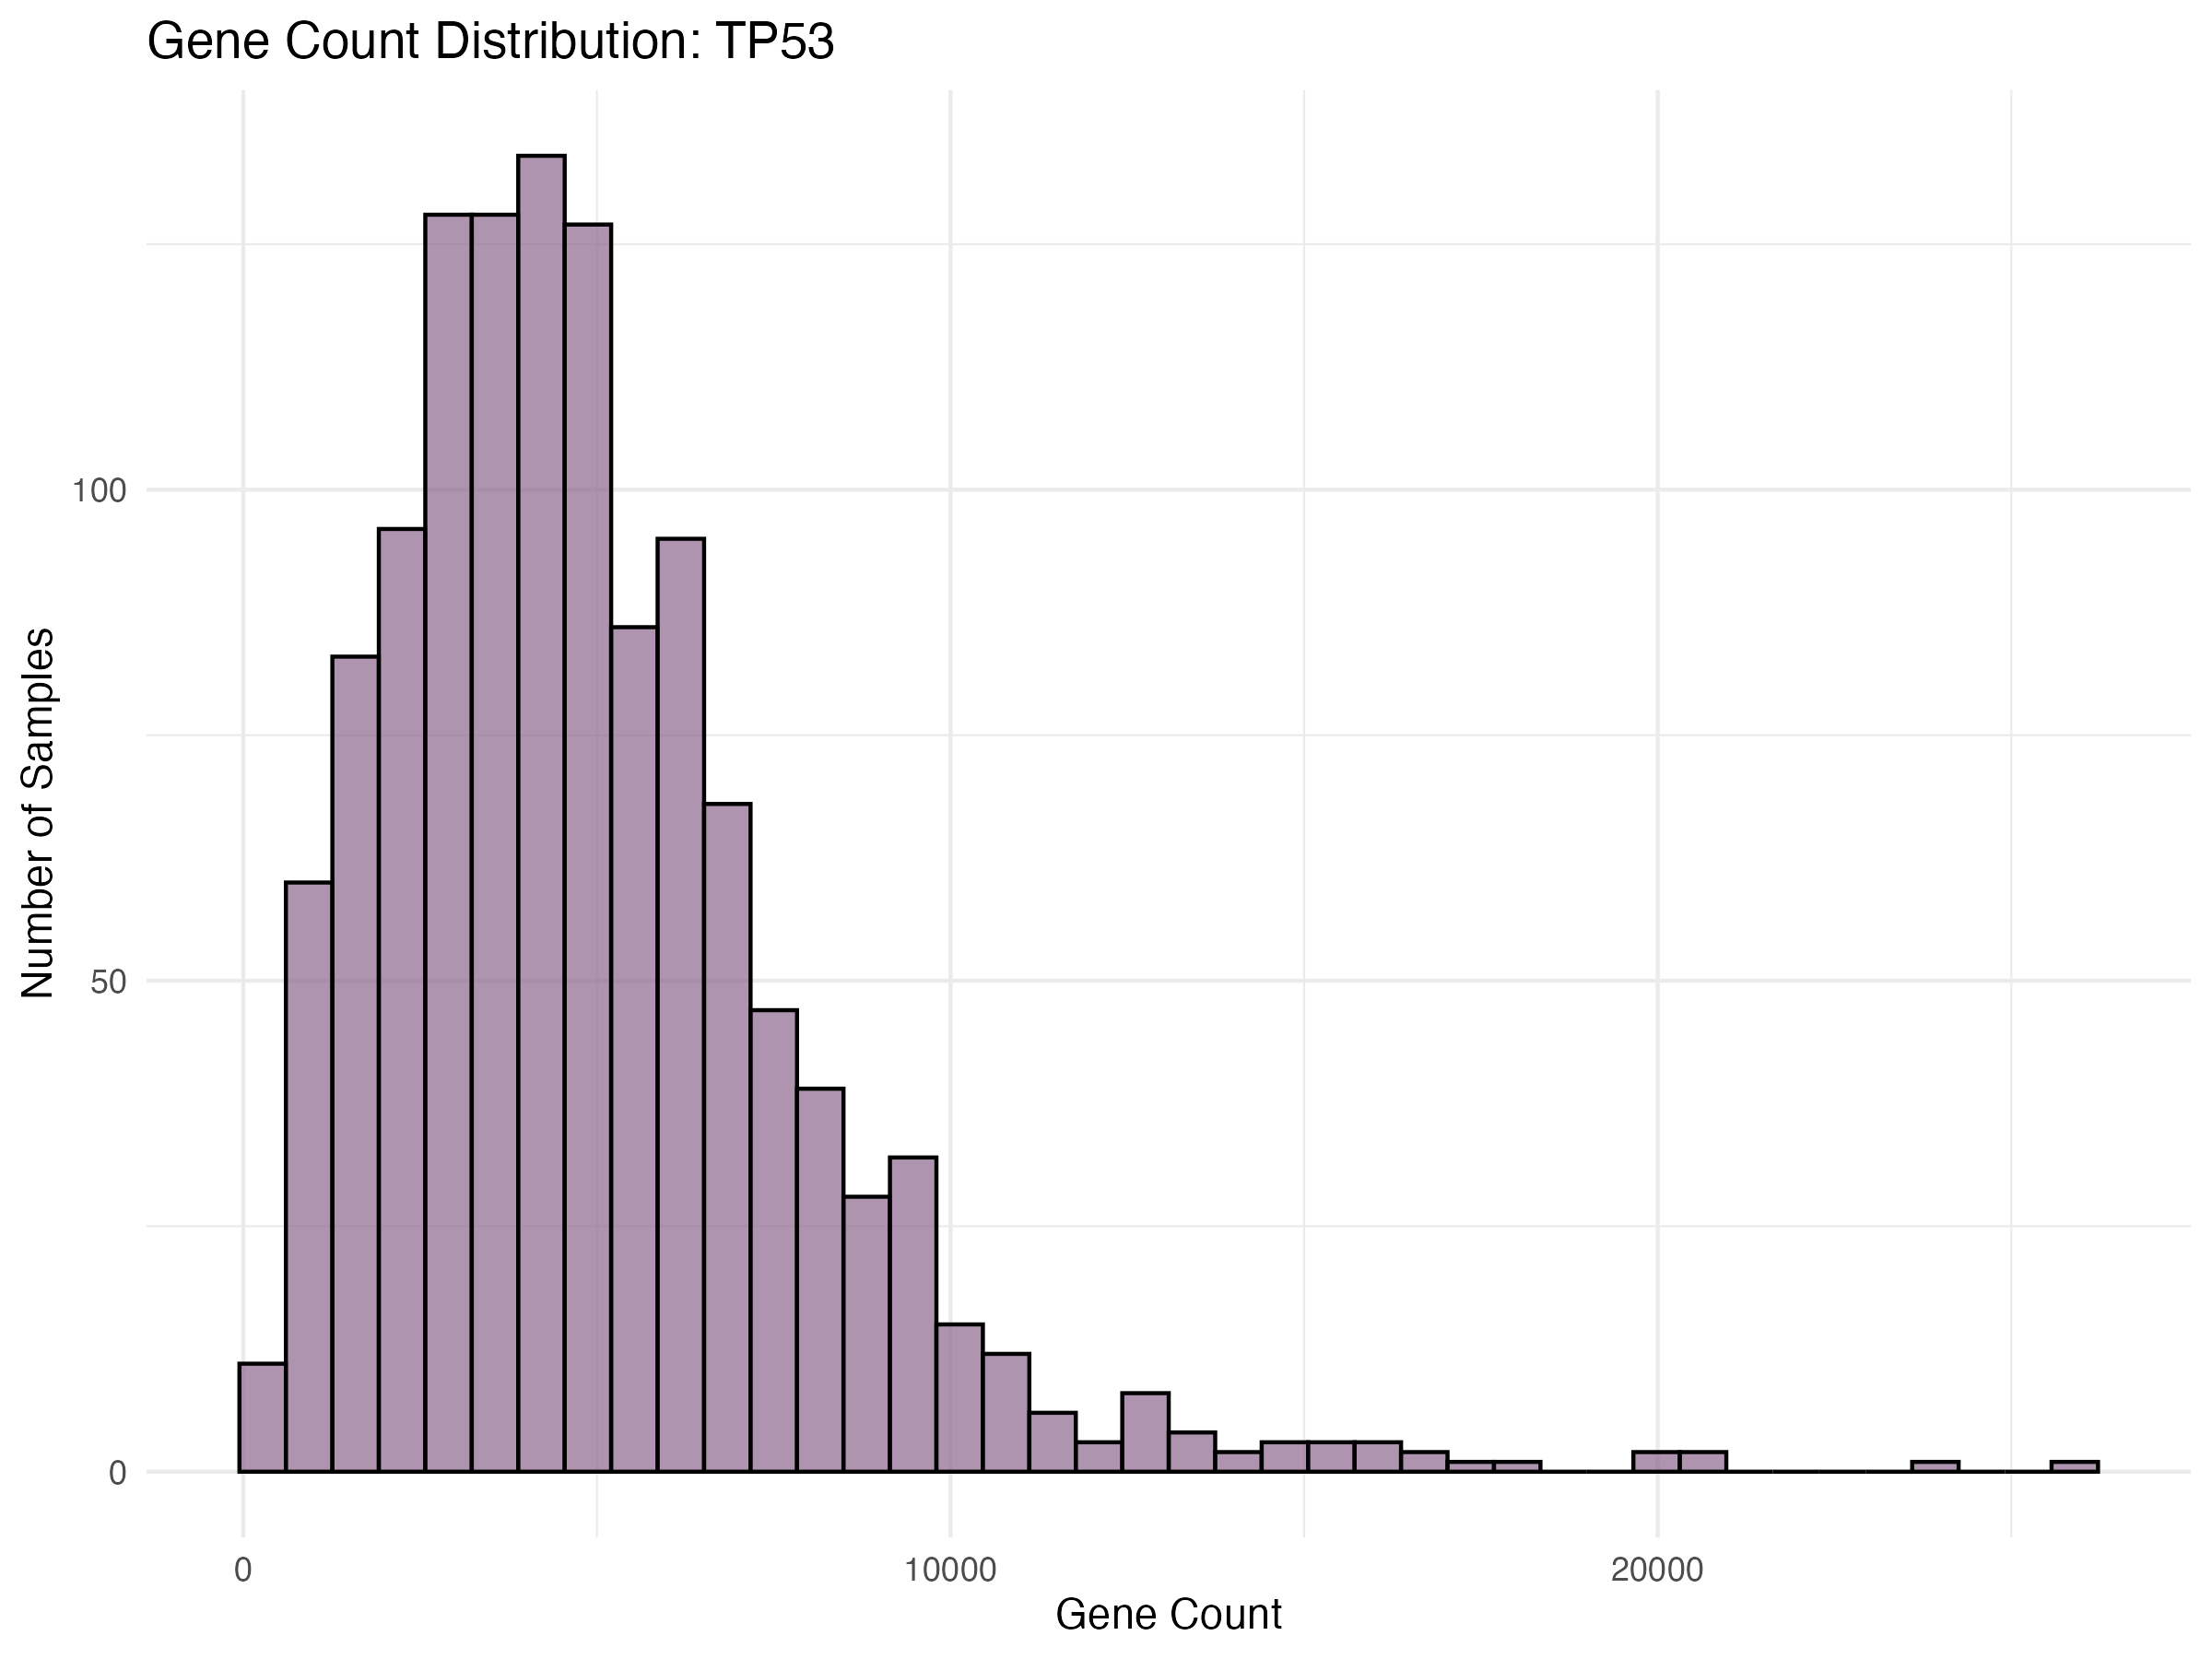
\includegraphics[width=0.75\textwidth]{final-project_histogram-plot.png}
    \caption{Histogram of TP53 Gene Counts}
    \label{fig:Histogram of TP53 Gene Counts}
\end{figure}

\subsection{Scatter Plot}
The scatter plot compares TP53 and PIK3CA counts for each sample. The fitted regression line has a positive slope, indicating that in general, samples with higher TP53 counts tend to have higher PIK3CA counts. However, the positive correlation does not guarantee that one causes another \cite{DartmouthCollegeMSHDSLectures}.

\begin{figure}[H]
    \centering
    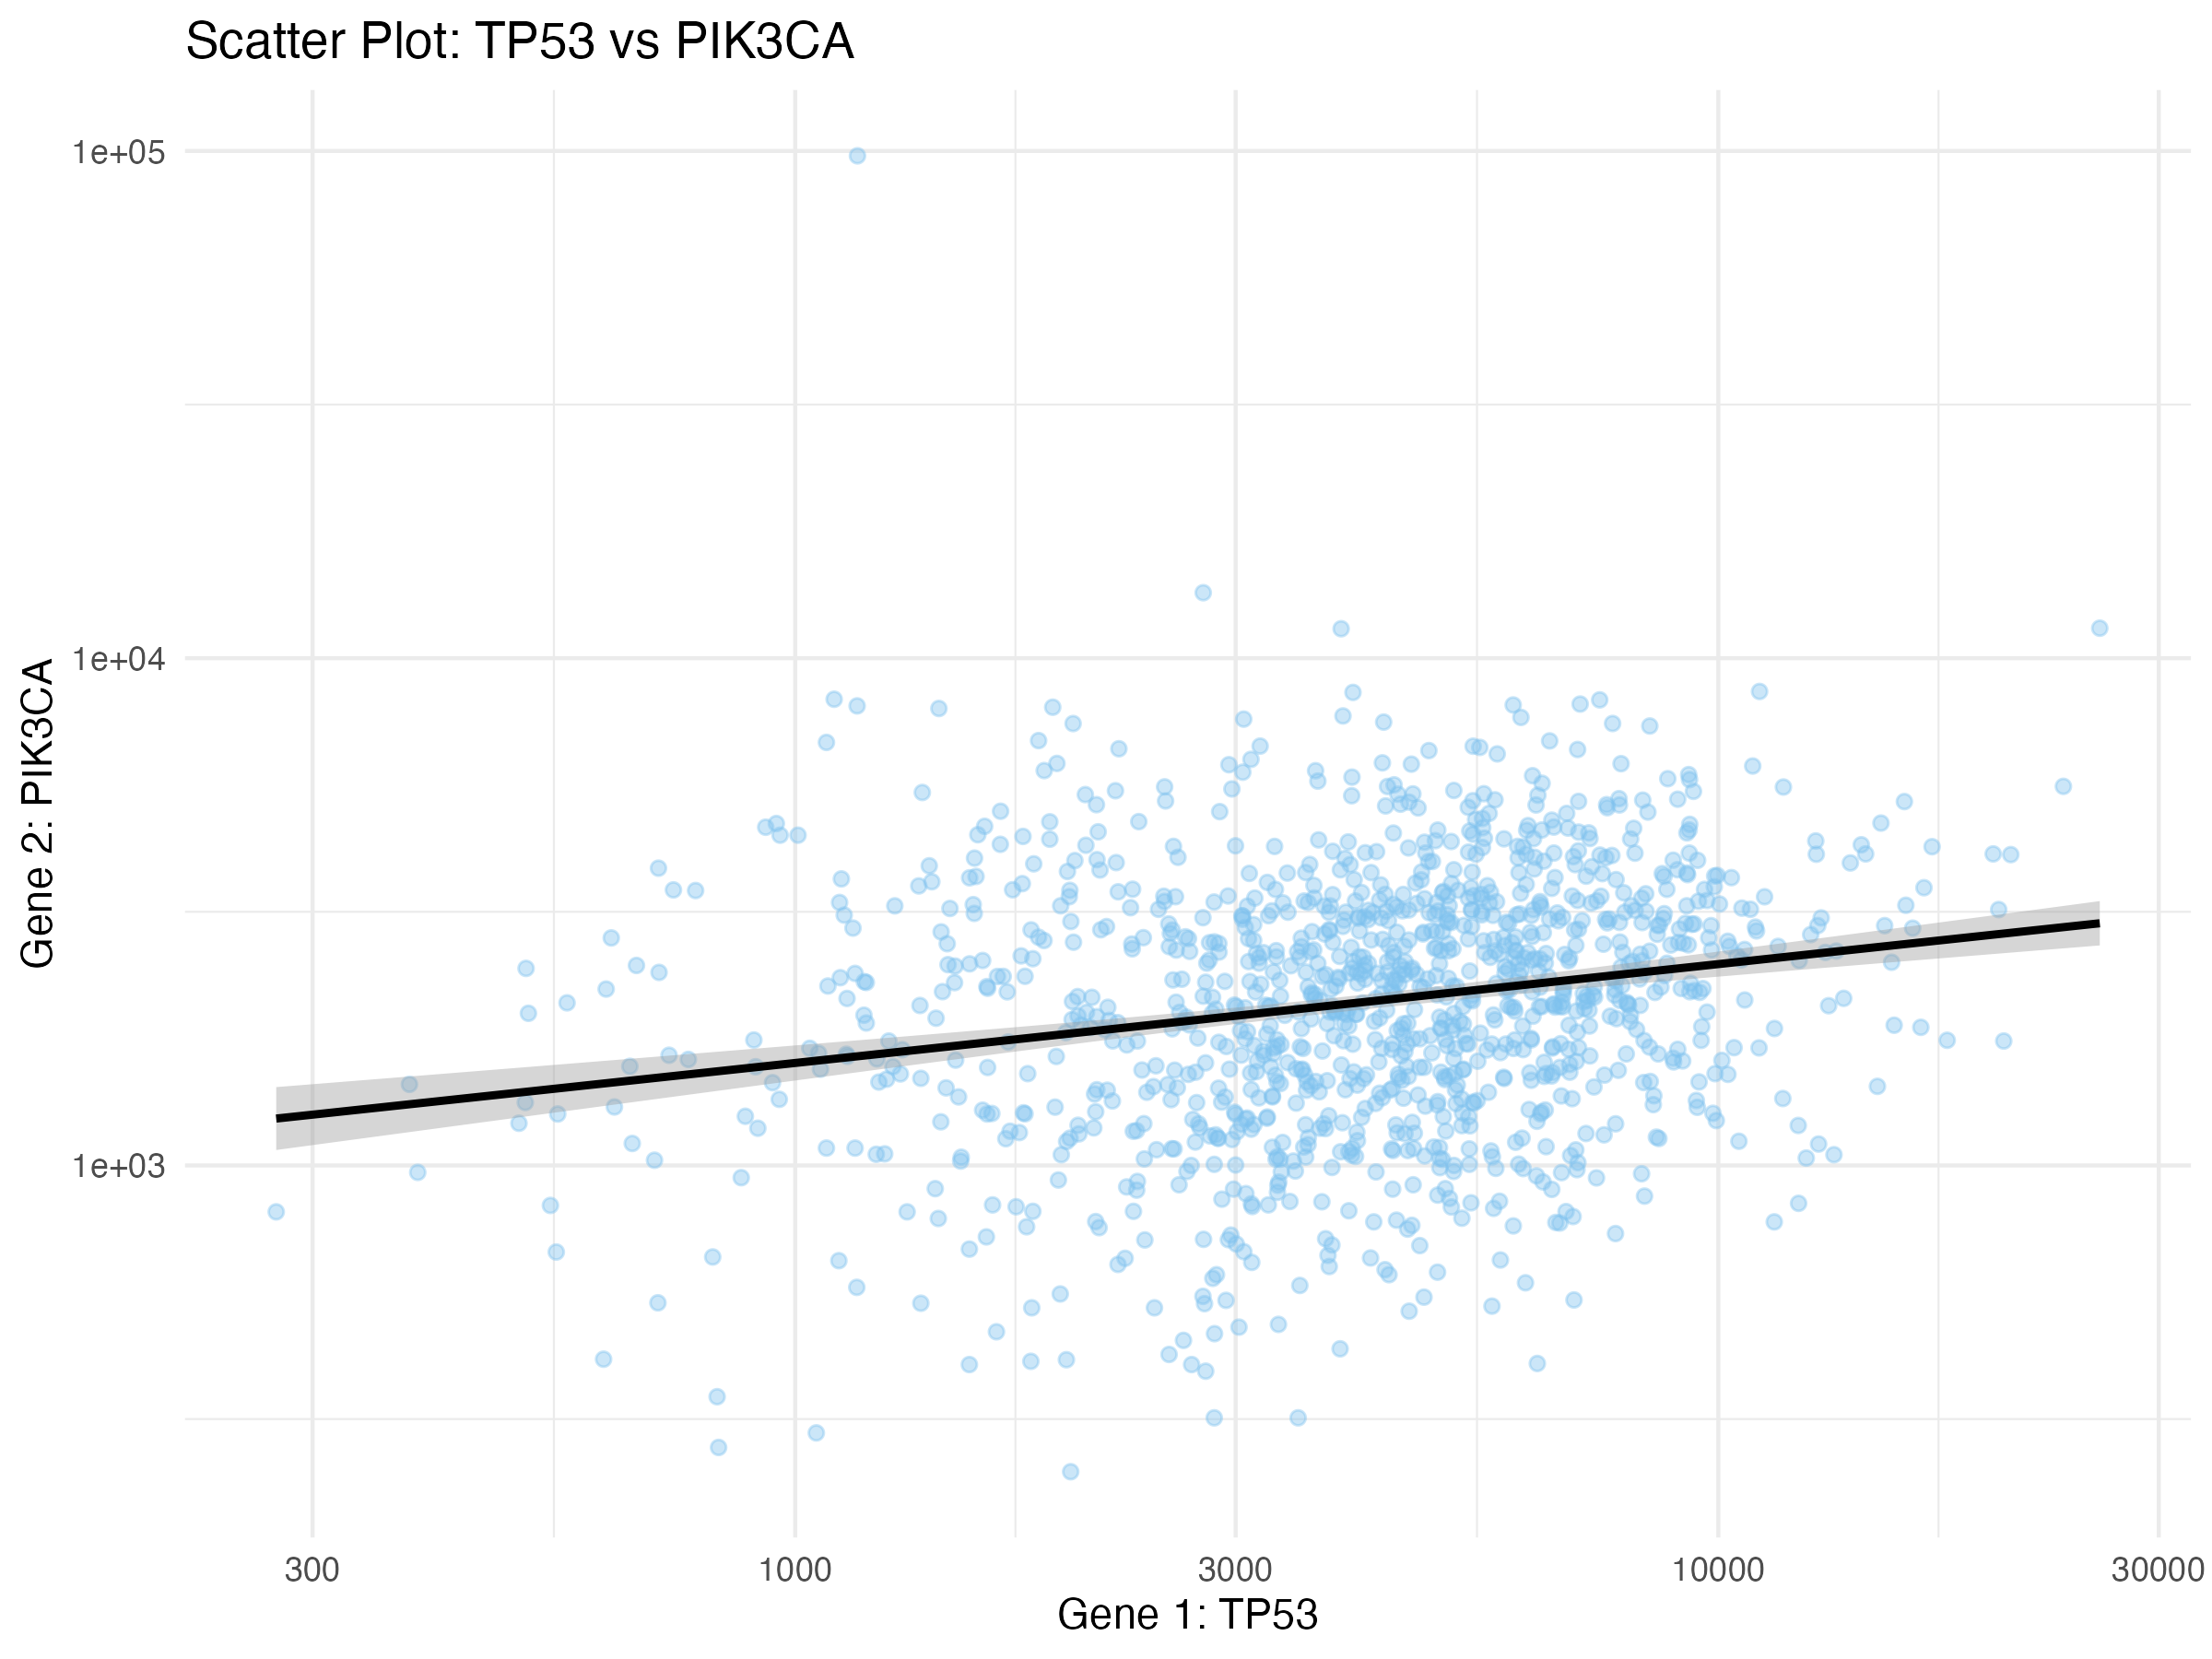
\includegraphics[width=0.75\textwidth]{final-project_scatter-plot.png}
    \caption{Scatter Plot of TP53 vs. PIK3CA Gene Counts}
    \label{Scatter Plot of TP53 vs. PIK3CA Gene Counts}
\end{figure}

\subsection{Violin Plot}
The violin plot shows the TP53 counts across the PAM50 breast cancer subtypes: Luminal A, Luminal B, HER2, Basal and Normal-like. Again, most samples have counts below 10000,with values mostly ranging from around 2000 to 4000. However, the LumA and Basal subtypes have counts exceeding 20000, unlike the others. 

\begin{figure}[H]
    \centering
    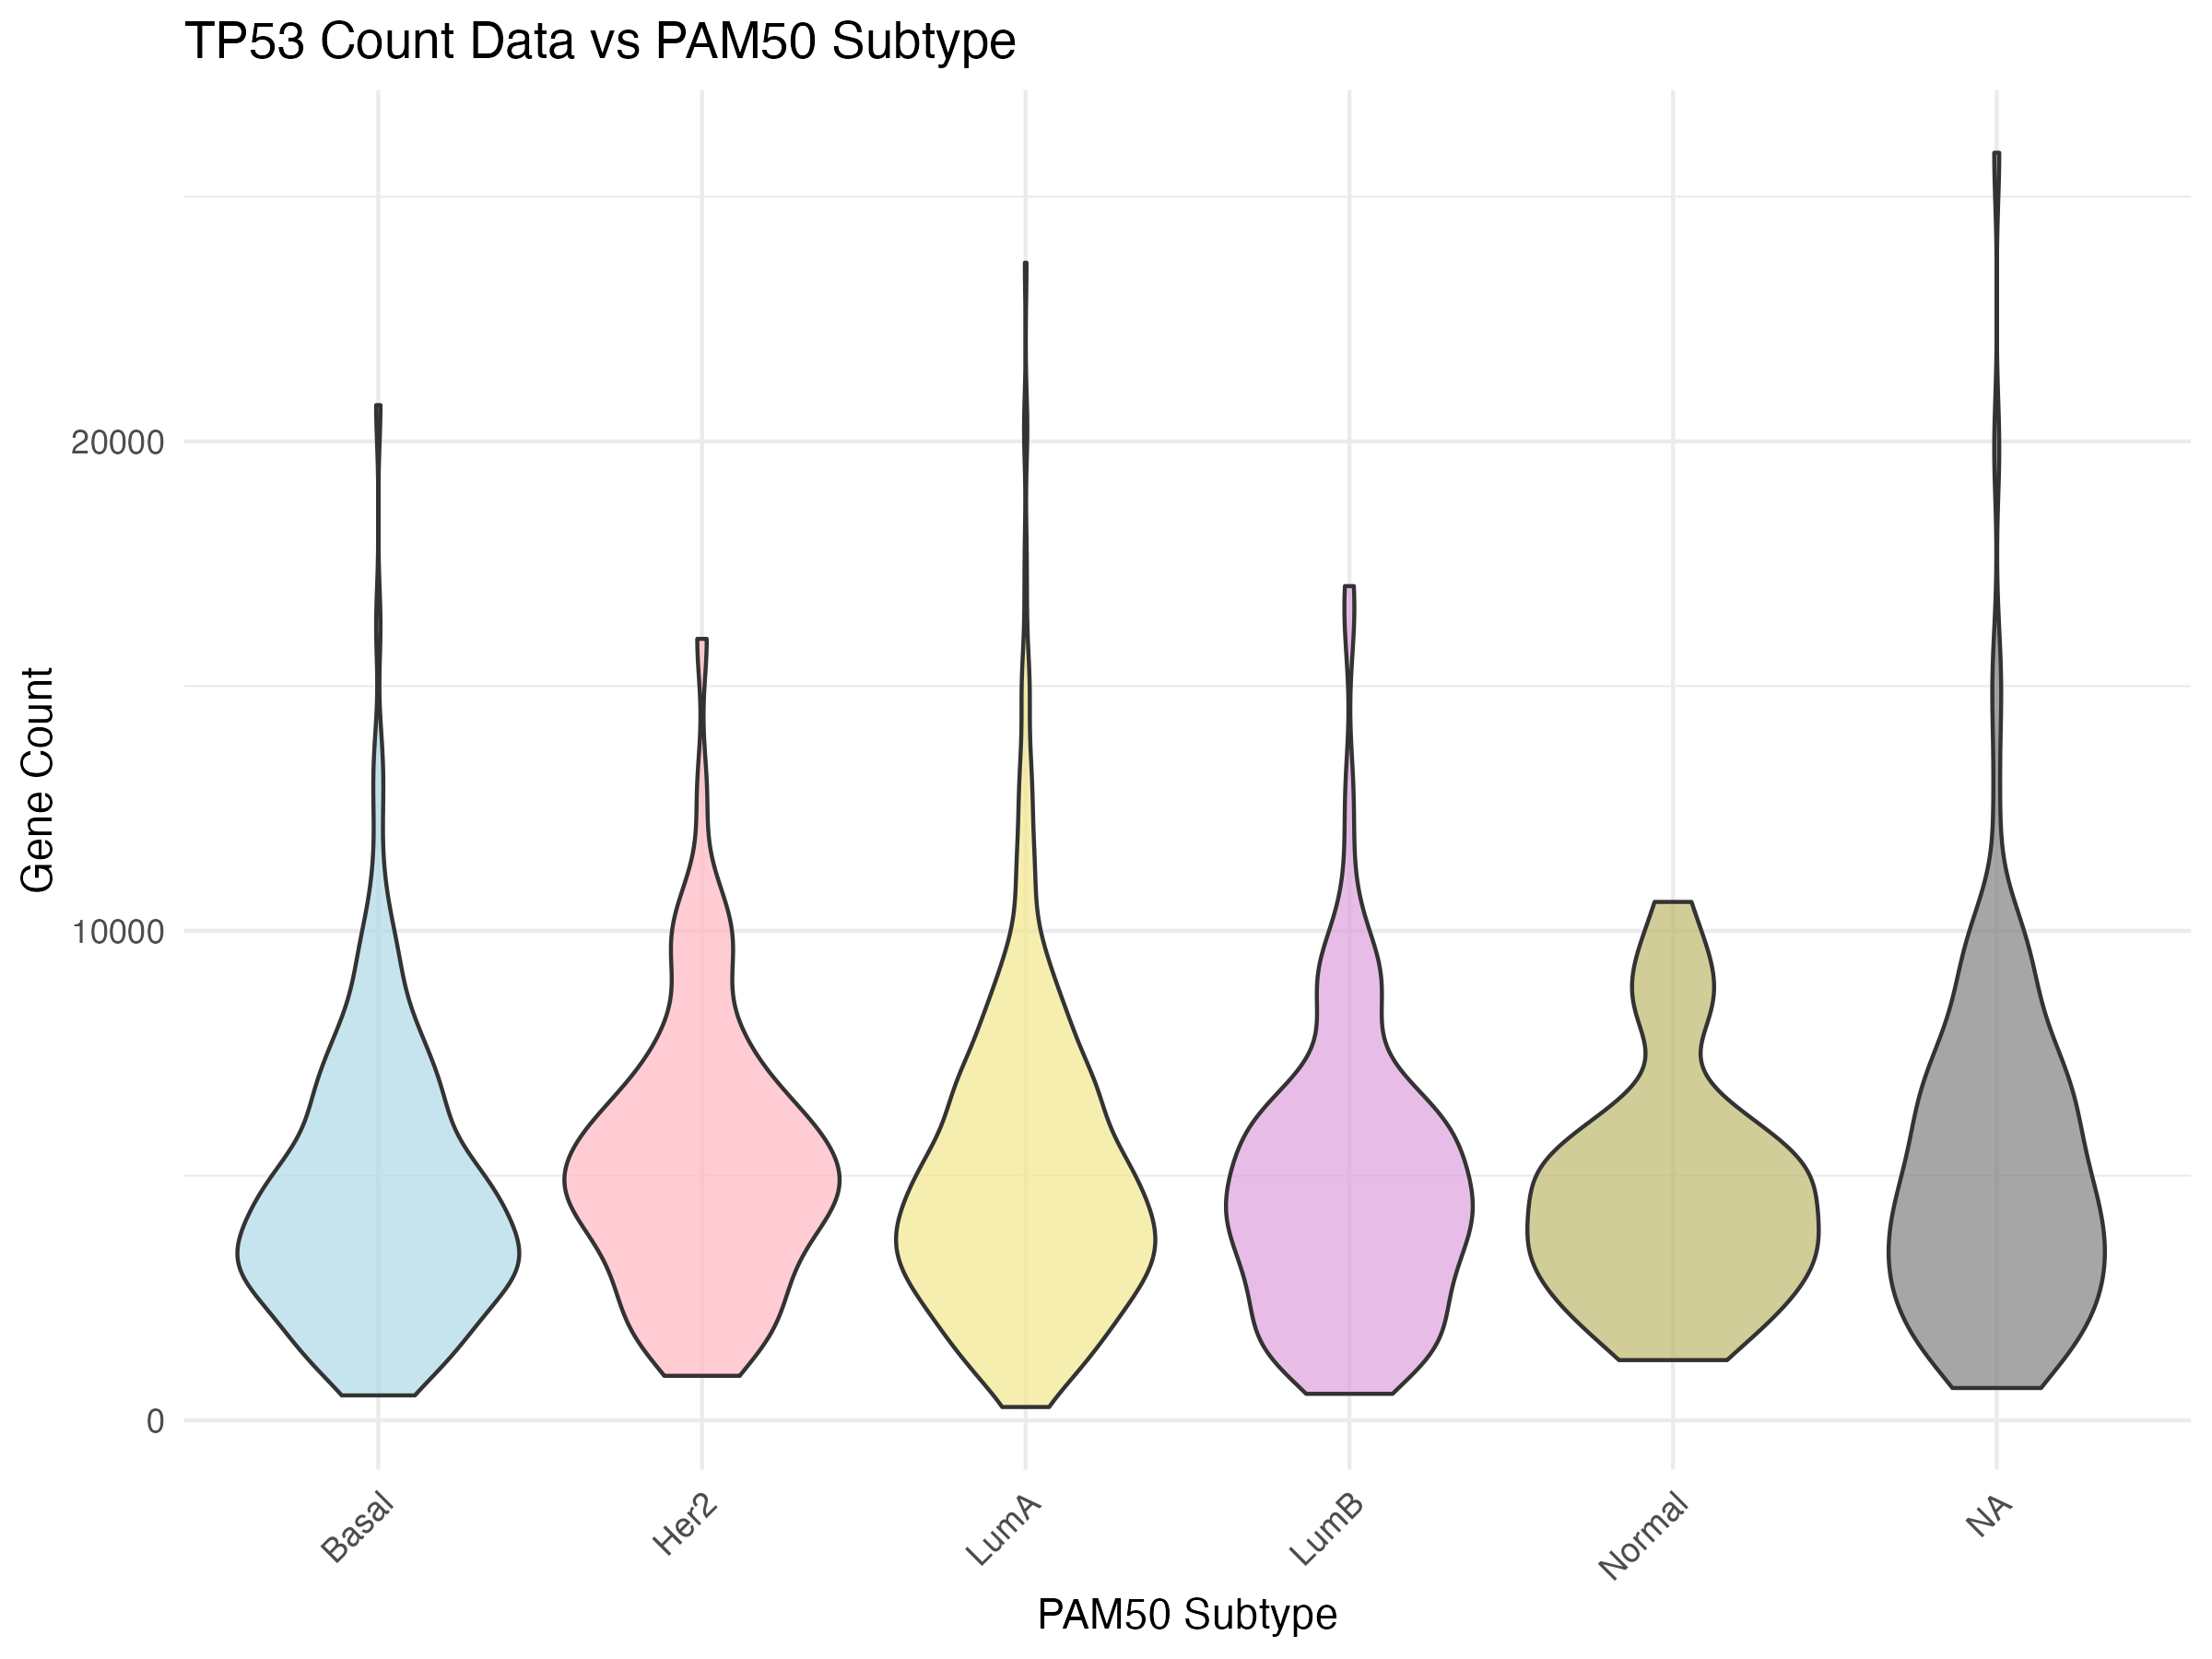
\includegraphics[width=0.75\textwidth]{final-project_violin-plot.png}
    \caption{Violin Plot of PAM50 Subtypes}
    \label{Violin Plot of PAM50 Subtypes}
\end{figure}

\subsection{Cumulative Distribution Function}
The cumulative distribution function (CDF) further illustrates the distrubution of TP53 gene counts. The median, corresponding to a cumulative probability of 0.50,  is approximately 5000 counts, indicating that at least half of the samples have fewer than 5000 TP53 gene counts. Additionally, the curve begins to plateau around 10000 counts, supporting the right-skewed histogram  \cite{DartmouthCollegeMSHDSLectures}. 

\begin{figure}[H]
    \centering
    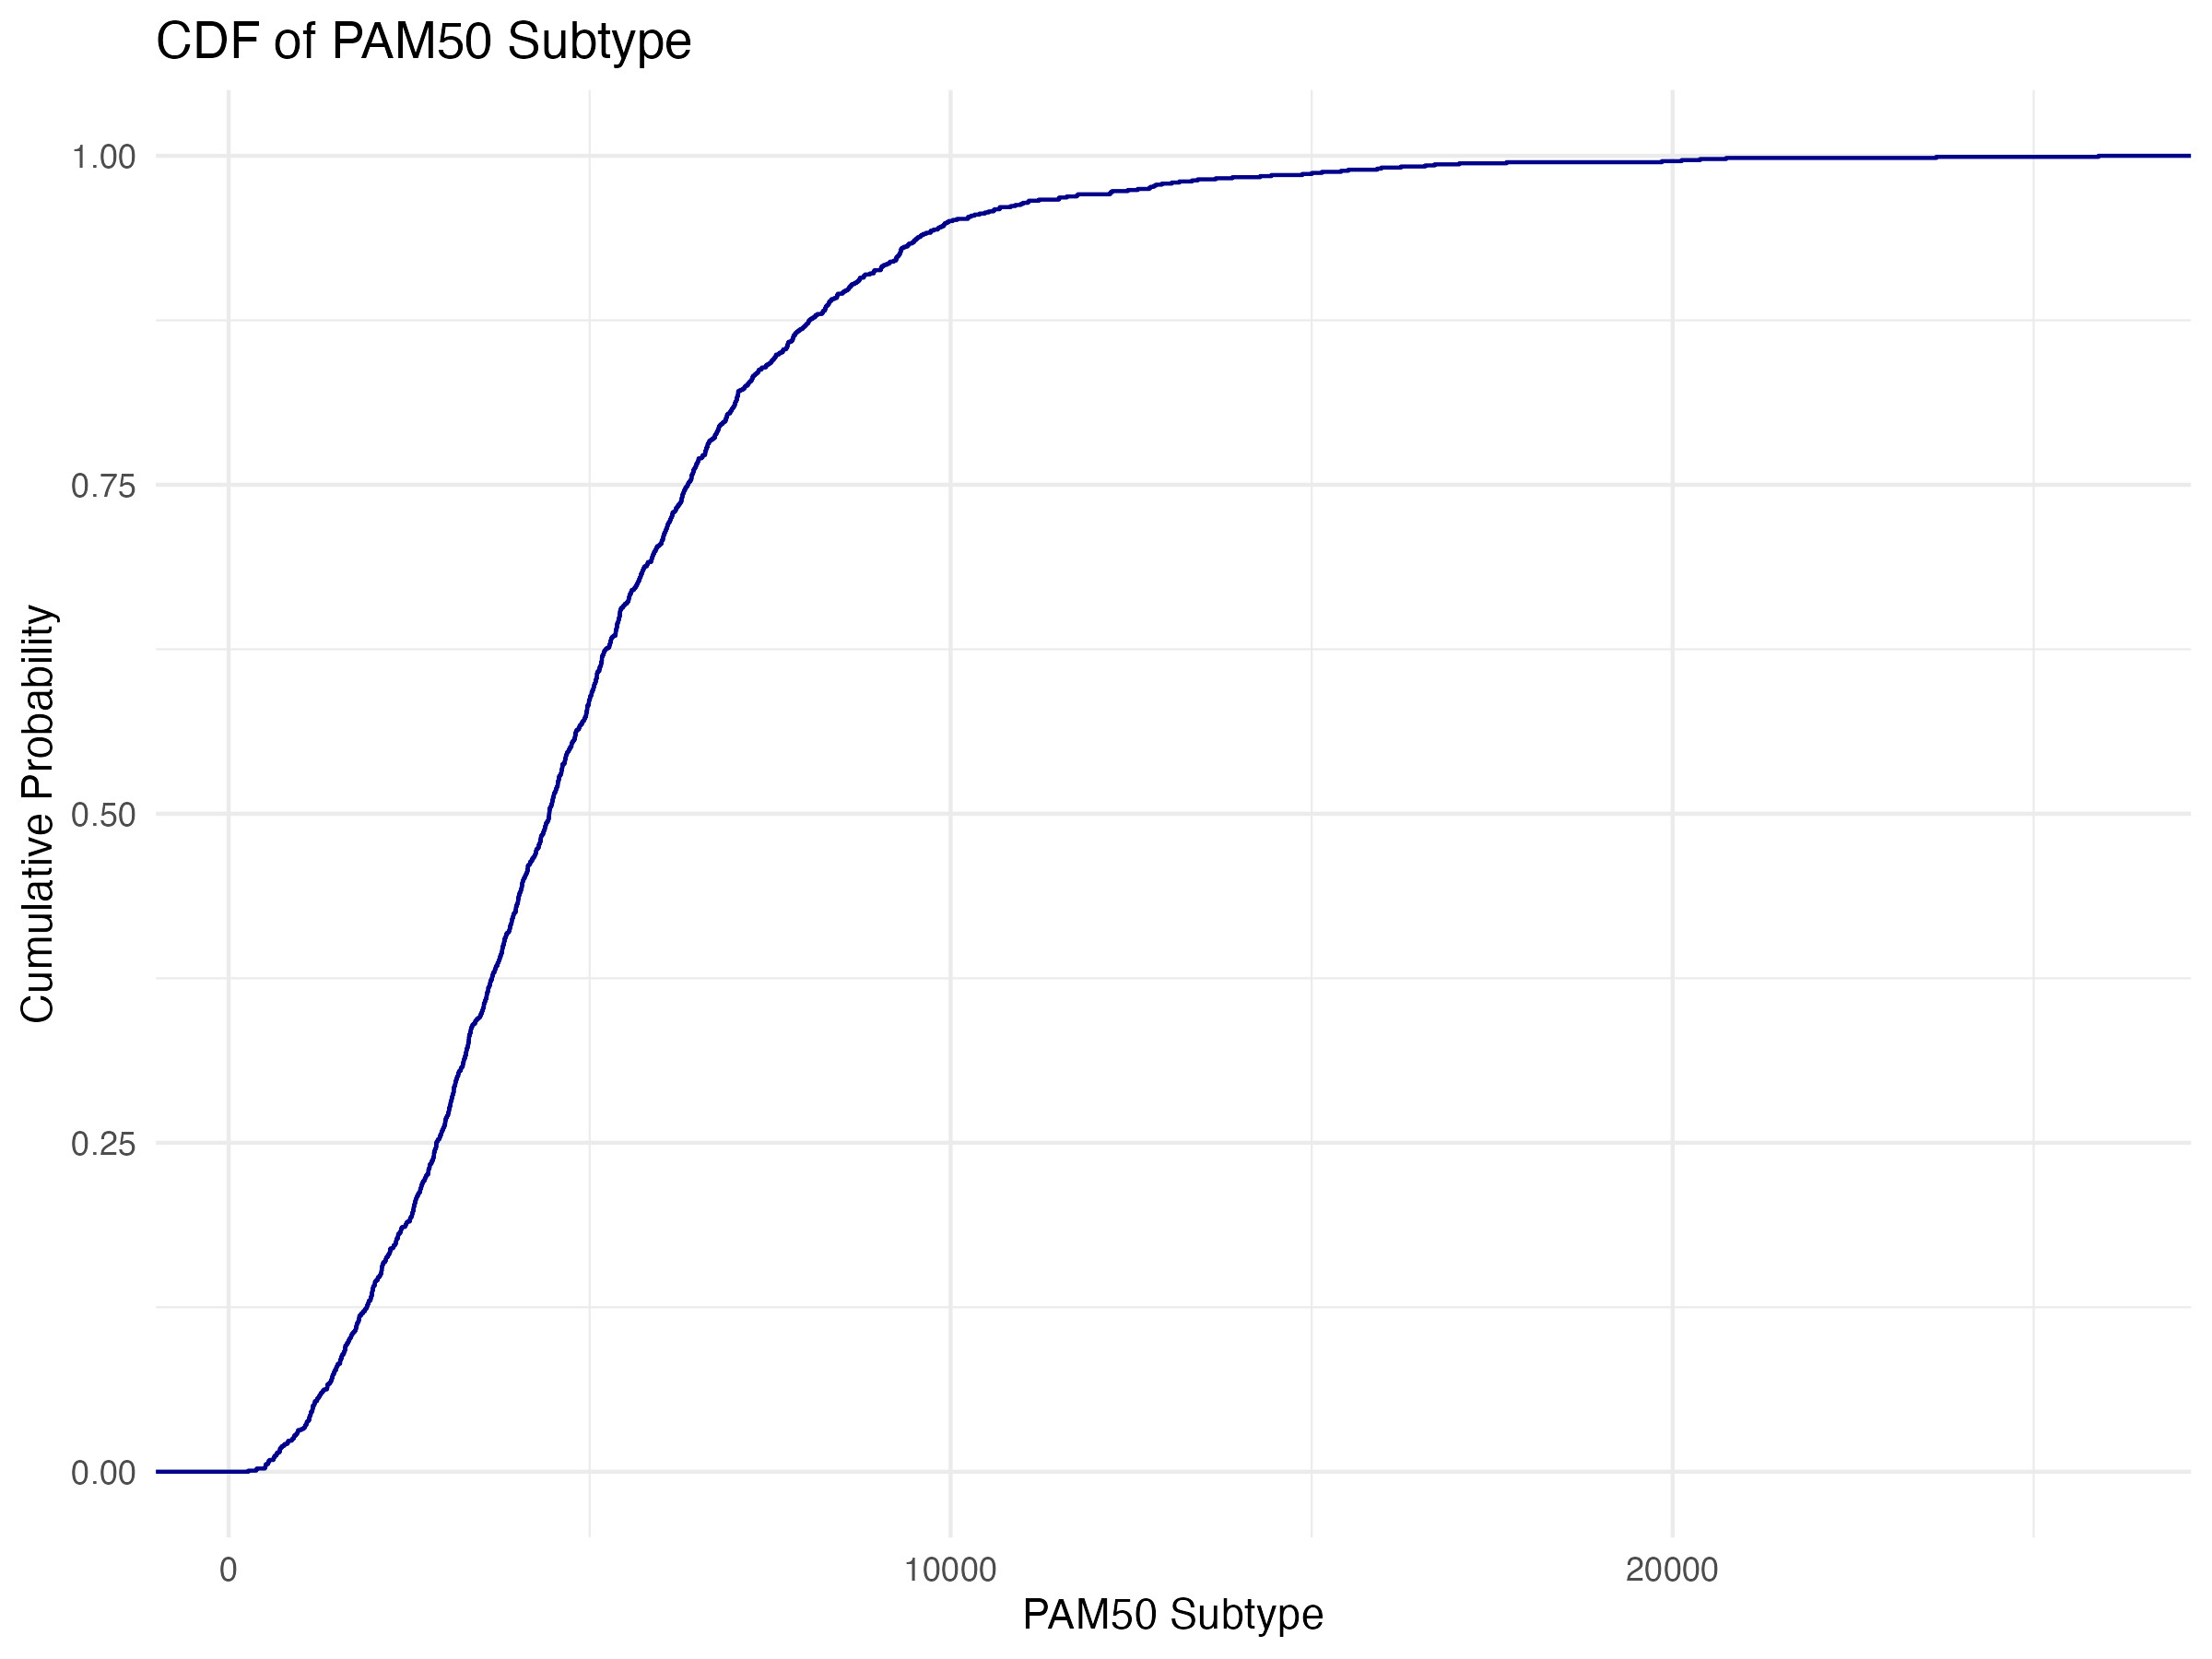
\includegraphics[width=0.75\textwidth]{final-project_cdf-plot.png}
    \caption{Cumulative Distribution Function (CDF) of TP53 Counts}
    \label{Cumulative Distribution Function of TP53 Counts}
\end{figure}

\subsection{Heatmap}
Finally, the heat map shows ten selected genes across all samples, with each sample's PAM50 subtype shown along the top. Most genes were specifically chosen to fall under the PAM50 subtype genes. Since the PAM50 subtype is represented by only 50 total genes, it makes sense that the samples are not visibly clustered by subtype \cite{DartmouthCollegeMSHDSLectures}. 

\begin{figure}[H]
    \centering
    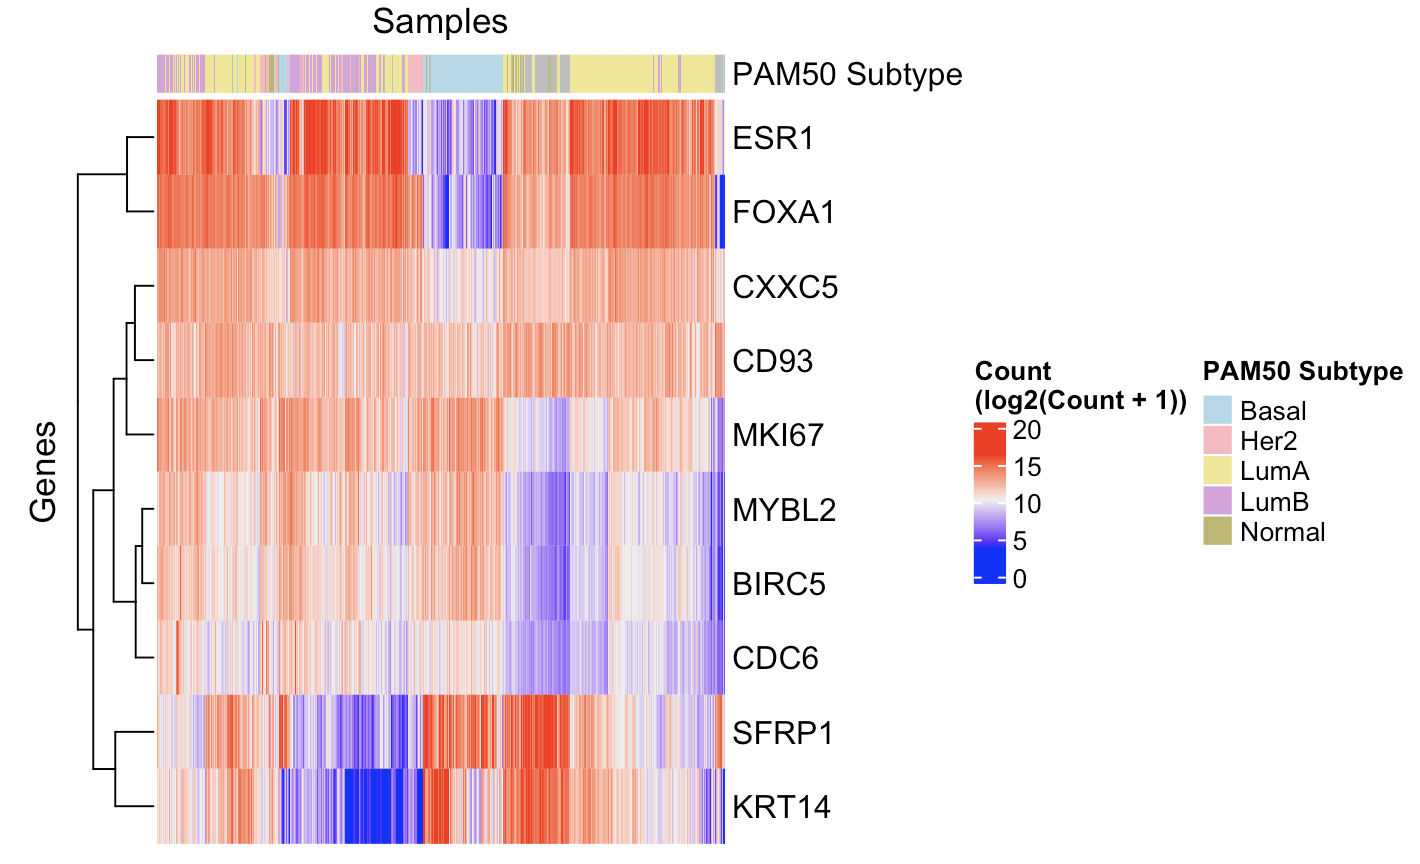
\includegraphics[width=0.75\textwidth]{heatmap_plot.png}
    \caption{Heatmap of 10 Selected Genes vs. PAM50 Subtype}
    \label{Heatmap of 10 Selected Genes vs. PAM50 Subtype}
\end{figure}

\subsection{Summary Statistics}
The following summary statistics display values for two co-variates: PAM50 Subtype and Age. PAM50 Subtype counts were first calculated, followed by summary statistic evaluation \cite{overleafTables}\cite{DartmouthCollegeMSHDSLectures}.

\begin{table}[H]
    \centering
    \begin{tabular}{ccc}
        \hline
        Subtypes & Counts \\ [0.5ex]
       \hline\hline
        Basal & 197  & \\
        Her2 & 82  & \\
        LumA & 571  & \\
        LumB & 209  & \\
        Normal & 40  & \\
        \hline
    \end{tabular}
    \caption{Summary of PAM50 Subtype Counts}
    \label{tab:pam50_counts}
\end{table}

\begin{table}[H]
    \centering
    \begin{tabular}{ccc}
       \hline
       Statistics & PAM50 & Age \\ [0.5ex]
       \hline\hline
       Min.  & 40.0  & 26.00 \\
       1st Qu.  & 94.5  & 48.00 \\
       Median  & 164.5  & 58.00 \\
       Mean  & 205.2  & 58.28 \\
       3rd Qu.  & 206.0  & 67.00 \\
       Max.  & 571.0  & 89.00 \\
       \hline
    \end{tabular}
    \caption{Co-variate Summary Statistics for PAM50 Subtypes and Age}
    \label{tab:covariates_summary}
\end{table}

\begin{thebibliography}{9}

\bibitem{NIH} 
National Cancer Institute - GDC Data Portal. \url{https://portal.gdc.cancer.gov/projects/TCGA-BRCA}

\bibitem{ensemblEnsembl}
Ensembl. \url{https://ensembl.org} (2026). Accessed: 2026-10-19.

\bibitem{medlineplusTP53Gene}
TP53 gene - MedlinePlus Genetics. \url{https://medlineplus.gov/genetics/gene/tp53/} (2026). Accessed: 2026-10-19.

\bibitem{medlineplusPIK3CAGene}
PIK3CA gene - MedlinePlus Genetics. \url{https://medlineplus.gov/genetics/gene/pik3ca/} (2026). Accessed: 2026-10-19.

\bibitem{overleafTables}
Tables - Overleaf. \url{https://www.overleaf.com/learn/latex/Tables%23Positioning_tables#Captions,_labels_and_references} (2026). Accessed: 2026-10-19.

\bibitem{DartmouthCollegeMSHDSLectures}
Fischer, S. (2026). Foundations of Data Science. Lecture Notes 1-5, Dartmouth College. Accessed: 2026-10.

\end{thebibliography}

\end{document}